\documentclass{clbeamer2024}

\usepackage{minted}

\usepackage{minted}
\setminted{
	breaklines=true,
	frame=single,
	bgcolor=lightgray,
	fontsize=\small,
	escapeinside=||
}

\usepackage{xcolor}
\definecolor{bg}{rgb}{0.95, 0.95, 0.92} % Couleur gris clair

\title{
	%
\includegraphics[width=0.5cm]{logos/IA1.png} \hfill
        Introduction à Gradle
	
\includegraphics[width=0.7cm]{logos/gradle.png} \hfill
}
\subtitle{Comprendre l'outil de build automation pour les projets Java et au-delà}
\author{Slimani Mohamed Amine}
\institute{EHTP}
\date{\today}

\begin{document}
	\setcounter{framenumber}{-1}
	\frame{\titlepage}
	
	
	
	% Sommaire
	\begin{frame}{Sommaire}
		\tableofcontents
	\end{frame}
	
	
	\section{Qu'est-ce que Gradle ?}
	\begin{frame}{Qu'est-ce que Gradle ?}
		\begin{itemize}
			\item \textbf{Définition} : Gradle est un outil de build automation open-source, utilisé pour automatiser la compilation, le test, et le déploiement de projets logiciels.
			\item \textbf{Objectif} : Simplifier et standardiser le processus de construction des projets.
			\item \textbf{Avantages} : Flexibilité, performance, et support multi-langages.
		\end{itemize}
	\end{frame}
	
	\section{Pourquoi utiliser Gradle ?}
	\begin{frame}{Pourquoi utiliser Gradle ?}
		\begin{itemize}
			\item \textbf{Flexibilité} : Supporte plusieurs langages de programmation (Java, Kotlin, C++, etc.).
			\item \textbf{Performance} : Utilise un cache intelligent pour accélérer les builds.
			\textbf{Écosystème} : Intégration avec de nombreux outils et plugins.
		\end{itemize}
	\end{frame}
	
	
	\section{Concepts de base de Gradle}
	\begin{frame}{Concepts de base de Gradle}
		\begin{itemize}
			\item \textbf{Projet} : Un projet Gradle représente une unité de travail (ex. une application, une bibliothèque).
			\item \textbf{Tâche} : Une action spécifique à exécuter (ex. compiler, tester).
			\item \textbf{Plugin} : Extensions qui ajoutent des fonctionnalités à Gradle.
			\item \textbf{Build Script} : Fichier de configuration (généralement `build.gradle`) qui définit les tâches et les plugins.
		\end{itemize}
	\end{frame}
	
	
	\section{Exemple de fichier build.gradle}
	\begin{frame}{Exemple de fichier build.gradle}
		\begin{exampleblock}{Fichier build.gradle pour un projet Java}
			
			\begin{center}
				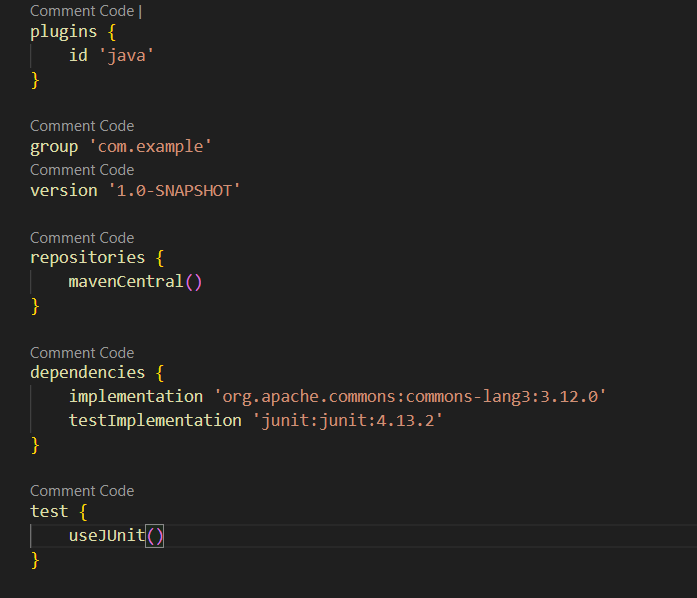
\includegraphics[width=0.7\textwidth]{images/code1.png}
			\end{center}
			
		\end{exampleblock}
	\end{frame}
	
	
	\section{Exemple de tâches Gradle}
	\begin{frame}[fragile]{Exemple de tâches Gradle}
		\begin{exampleblock}{Commandes Gradle courantes}
			\begin{minted}[fontsize=\scriptsize]{bash}
# Compiler le projet
gradle build
				
# Exécuter les tests
gradle test
				
# Nettoyer le projet
gradle clean
				
# Exécuter une tâche spécifique
gradle myTask
			\end{minted}
		\end{exampleblock}
	\end{frame}
	
	
	\section{Bonnes pratiques}
	\begin{frame}{Bonnes pratiques}
		\begin{itemize}
			\item \textbf{Modularisation} : Diviser le projet en plusieurs modules pour une meilleure gestion.
			\item \textbf{Utilisation des plugins} : Utiliser des plugins officiels pour des fonctionnalités standard.
			\item \textbf{Gestion des dépendances} : Utiliser des dépôts fiables comme Maven Central.
		\end{itemize}
	\end{frame}
	
	
	\section{Outils pour travailler avec Gradle}
	\begin{frame}{Outils pour travailler avec Gradle}
		\begin{itemize}
			\item \textbf{IDE} : Intégration avec des IDE comme vs Code, IntelliJ IDEA et Eclipse.
			\item \textbf{Gradle Wrapper} : Permet d'exécuter Gradle sans installation préalable.
			\item \textbf{Documentation} : Consulter la documentation officielle pour des guides détaillés.
		\end{itemize}
	\end{frame}
    
    
    \section{Défis de Gradle}
    \begin{frame}{Défis de Gradle}
    	\begin{itemize}
    		\item \textbf{Courbe d'apprentissage} : La syntaxe Groovy ou Kotlin peut être complexe pour les débutants.
    		\item \textbf{Performance} : Les builds peuvent être lents pour les très grands projets.
    		\item \textbf{Compatibilité} : Assurer la compatibilité avec les anciennes versions de Gradle.
    	\end{itemize}
    \end{frame}
    
    
    \section{Pourquoi c'est important ?}
    \begin{frame}{Pourquoi c'est important ?}
    	\begin{itemize}
    		\item Gradle est un outil essentiel pour automatiser et standardiser les builds de projets logiciels.
    		\item Il permet de gérer efficacement les dépendances et les tâches de construction.
    		\item Comprendre Gradle est crucial pour les développeurs Java et au-delà.
    	\end{itemize}
    \end{frame}
	
	
	\begin{frame}{Résumé}
		\textbf{Gradle} est un outil puissant pour l'automatisation des builds, offrant flexibilité, performance, et un écosystème riche.  
		Explorez, apprenez, et utilisez Gradle pour améliorer vos projets ! 
	\end{frame}
	

	
\end{document}
